\newpage
\section{Diskussion}
\label{sec:Diskussion}
Der Diodenlaser konnte fachgemäß in Betrieb genommen werden, wie die Ergebnisse aus den Abschnitten (\ref{sec:über1}) und (\ref{sec:über2}) beweisen. Die erwarteten Effekte, also Specklebildung ab
Schwellenstrom und die Fluoreszenz des Rubidium sind beide eingetroffen.
Das Bild des Absorptionsspektrum aus der Abbildung (\ref{fig:mess4}) stimmt mit dem aus der Theorie erwarteten Ergebnis (siehe Abbildung (\ref{fig:absot})) überein.
\begin{figure}[h!]
  \centering
  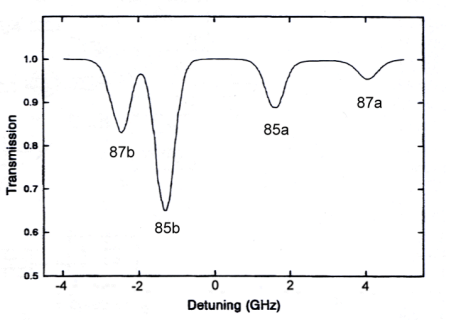
\includegraphics[scale=0.7]{fig/absot.png}
  \caption{Erwartetes Absorptionsspektrum \cite[13]{Anleitung4}.}
  \label{fig:absot}
\end{figure}
\FloatBarrier
\noindent Die Linien aus Abbildung (\ref{fig:mess4}) können demnach von links nach rechts den Übergangen 87b, 85b, 85a, 87a zugeordnet werden können.
Das Experiment ist gelungen und alle aufgestellten Vermutungen konnten gezeigt werden.
